\section{Fazit}

Das redaktionelle Konzept beschreibt die vorgesehenen Inhalte je Seite in Kurzform. Au�erdem wird hierbei auch eine Richtlinie zur Aktualisierungsh�ufigkeit je Seite vorgegeben (unterst�tzt SEO). Somit wird erreicht, dass der redaktionelle Verantwortliche eine kompakte Anleitung zur Pflege der Website erh�lt.

Beim Navigationskonzept wurden die wichtigsten Navigationselemente beachtet. Hervorzuheben sind hier die "`Breadcrumb"'-Navigation und die Implementierung von mod\_rewrite (Abbildung ~\ref{abb:htaccess}, Seite ~\pageref{abb:htaccess}).

Durch die Formatierung der Website mithilfe von CSS kan der Redakteur sich im Wesentlichen auf die Inhalte bzw. auf die in einem zu erstellenden Handbuchs korrekte Auszeichnung mit relativ einfachen HTML--Tags konzentrieren, und nicht auf die Gestaltung der Website.

\begin{figure}[h]
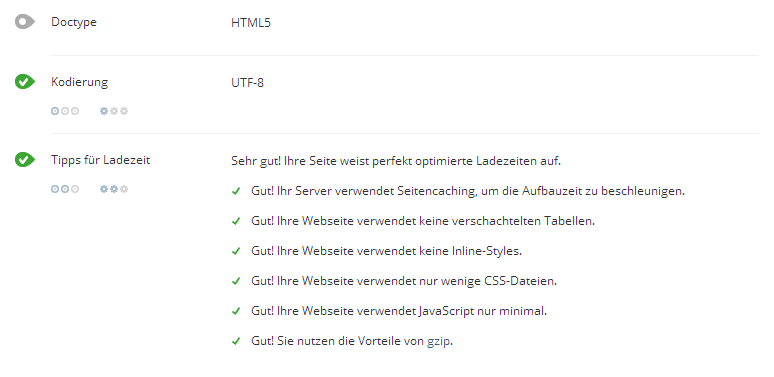
\includegraphics[width=\hsize]{scr_woorank_performance.png}
\caption{Screenshot: Performance}
\label{scr:performance}
\end{figure}

Die Website erf�llt die gestellten Anforderungen vollst�ndig. So bescheinigt, wie die Abbildungen~\ref{scr:performance} und~\ref{scr:mobile} zeigen, das SEO--Analyse--Tool \code{woorank.com}, dass z.B. nicht-funktionalen Anforderungen wie die Performance der Site sehr gut erf�llt werden. Durch den Einsatz von Media--Queries wird eine gro�e Bandbreite von Ger�ten unterst�tzt. Optimierungspotential ergibt sich hier noch durch eine m�gliche auf die Bildschirmgr��e abgestimmte Auslieferung der Grafiken. Dies w�rde aber den in der Aufgabenstellung vorgegebenen Rahmen an notwendigem Know--How f�r die Pflege der Website bzw. den Verzicht auf externe Hilfsmittel sprengen. 

\begin{figure}[h]
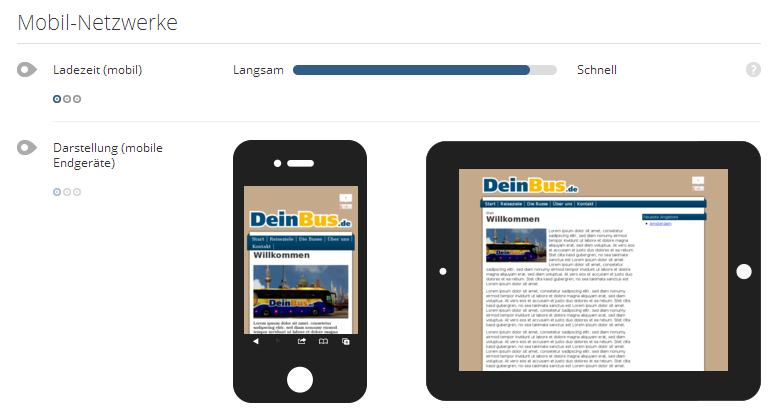
\includegraphics[width=\hsize]{scr_woorank_mobile_performance.png}
\caption{Screenshot: Mobile Ger�te}
\label{scr:mobile}
\end{figure}

Somit liegt ein n�chster m�glicher Schritt nahe, n�mlich die Verwendung eines Content-Management-Systems (CMS). Dies erm�glicht das einfache Bearbeiten der Seiteninhalte mithilfe eines WYSIWYG-Editors (keine Code-Kenntnisse notwendig) und das Aufrechterhalten eines konsistenten Designs. 

Die Navigation kann auf mehrere Ebenen und Elemente verteilt werden und aktualisiert sich selbst�ndig. Der Administrationsaufwand wird somit stark reduziert und trotzdem f�llt es erstaunlich leicht die Funktionen der Website durch vorgefertigte Module zu erweitern. So ist es ebenfalls m�glich einen Weblog zu betreiben welcher mit Facebook und anderen Social-Media-Diensten integriert werden kann. 

Urspr�nglich als Weblog-System zu gro�er Bekanntheit gelangt, kann Wordpress heute als einfaches und komfortables CMS genannt werden. F�r komplexere Anwendungsf�lle eignet sich Drupal oder Typo3.

Abschlie�end l�sst sich feststellen, dass der Betrieb einer Website heute mit den kostenlos angebotenen und doch professionellen Systemen deutlich besser und einfacher m�glich ist, als mit selbst erstelltem Code. Trotzdem werden auch hier ein redaktionelles-- und ein Navigationskonzept ben�tigt. Beim Design w�re abzuw�gen, ob man eine fertige, zur Firma passende Designvorlage\footnote{je nach System gibt es eine gro�e Auswahl von Designvorlagen, bzw. Themes oder auch Templates} �bernimmt, oder ob man sich von einem Dienstleister ein perfekt passendes Design f�r das gew�hlte CMS erstellen l�sst.


